% \documentclass[a4paper,fleqn]{cas-sc}
\usepackage[authoryear,longnamesfirst]{natbib}
\usepackage{amsmath,amssymb}
\usepackage{graphicx}
\usepackage{url}
\usepackage{float}

\newtheorem{theorem}{Theorem}
\newtheorem{proposition}[theorem]{Proposition}
\newproof{proof}{Proof}




% \begin{document}
% \let\WriteBookmarks\relax
% \def\floatpagepagefraction{1}
% \def\textpagefraction{.001}

% \shorttitle{Conformal envelopes}
% \shortauthors{YOUR NAME}

% \title[mode=title]{Conformal envelopes: class specific conformal prediction sets with missing scores}

% \author[1]{Nizalia Siddiqui}
% \cormark[1]
% \fnmark[1]
% \ead{nizaliasiddiqui25@gmail.com}
% \credit{Methodology, Software, Validation, Formal analysis, Investigation, Writing -- original draft}

% \author[1]{Clovis Galiez}
% \ead{clovis.galiez@univ-grenoble-alpes.fr}
% \credit{Conceptualization, Methodology, Supervision, Writing -- review and editing}

% \affiliation[1]{organization={Univ. Grenoble Alpes, CNRS, Grenoble INP, LJK},
%             addressline={ 150 Place du Torrent, Universitaire de Saint-Martin-d'H\`eres},
%             postcode={38401},
%             city={Grenoble},
%             country={France}}
% \cortext[1]{Corresponding author}
% \fntext[1]{Present address: Islamabad, Pakistan}

% %%%%%%%%%%%%%%%%%%%%%%%%%%%%%%%%%%%%%%%%%%%%%%%%%%%%%%%%%%%%%%%%%%%%%%%%%%%%%%%%%%%%%%%%%%%

% \begin{abstract}
Conformal prediction uses the output of a trained predictor and returns a prediction set that contains the true label 
with a chosen probability. When there are several predictors scoring each candidate class, the scores have to be 
combined, and the way they are combined influences the size of the sets. We present class specific conformal envelopes 
for classification. For each class, the shape of an envelope in the space of the score vectors is learned on one part of 
the calibration data of that class, and its size is scaled on the other part. Here we propose three envelope construction 
methods: a collapsed envelope that averages the scores, a radial envelope whose boundary depends on the direction of the 
score vector, and a strip envelope that bounds each score given the value of another score. All three methods only use 
the observed scores of a sample, so samples with missing scores still receive prediction sets. We show that when the 
samples of a class are exchangeable and the missingness has the same distribution in the calibration and test data, the 
sets have at least the nominal level of class conditional coverage. These constructions are implemented in an open source 
Python package. In experiments on simulated data with missing scores and on football player classification with four 
roles and with twenty positions, the average coverage of all three constructions is between 0.899 and 0.903 for a 
target of 0.9, the set sizes are similar, and no construction is best in every experiment.

\end{abstract}

\begin{highlights}
\item Class specific conformal envelopes built from scores from several predictors
\item Three envelope construction methods (collapsed, radial, strip)
\item Class conditional coverage guarantee within each class under exchangeability
\item Samples with missing scores still receive prediction sets
\item Open source Python package; coverage near 90\% on simulated and football data
\end{highlights}

\begin{keywords}
conformal prediction \sep classification \sep missing scores \sep prediction sets \sep software
\end{keywords}



% \maketitle

% \section{Introduction}\label{sec:intro}

Conformal prediction can be used to turn the output of any trained predictor into a prediction set that contains the 
true label with a defined probability, and it needs no assumption on the distribution of the data except exchangeability 
\citep{vovk2005algorithmic,shafer2008tutorial,angelopoulos2023conformal}. In classification, the set is built from a 
nonconformity score, which measures how badly a candidate label agrees with an input. The coverage guarantee holds 
for every choice of score, but the choice affects the size of the sets. A poorly chosen score gives sets that are valid 
but too large to be useful.

Several predictors also often score each candidate class, for example classifiers with different models or different input 
features. These candidate scores are then combined into a vector, which is aggregated into a single scalar score. A 
fixed rule such as the mean treats all predictors in the same way, even though they can differ in reliability and they 
can be dependent on other predictors. Mostly the methods for conformal aggregation combine the prediction sets of the 
individual predictors \citep{gasparin2024merging,yang2024selection}, or project the score vector on one weighted direction 
\citep{luo2024weighted}. Instead of this, \citet{ochoarivera2024conformal} work in score space. They 
define a quantile envelope for the multivariate score as the intersection of half spaces along random directions, learn 
its shape on one part of the calibration data and scale it on the other part, which gives marginal coverage.

In this paper we build on this idea in a classification setting. The envelope is learned separately for each class, 
from the score vectors of the samples of that class, so that the coverage statement holds for each class. This is known 
as Mondrian conformal prediction \citep{vovk2005algorithmic}. We present three envelope constructions that share the same 
two stage calibration: a collapsed envelope, which averages the scores, a radial envelope, in which the boundary changes 
with the direction of the score vector, and a strip envelope, which bounds each coordinate given the value of another 
coordinate. The radial and strip envelopes are not intersections of half  spaces, and all three constructions use only 
the observed scores of a sample, so a score vector with missing entries can still be assigned a prediction set.


Our contributions are the radial and strip constructions, the handling of missing scores, an open source Python package that 
implements them (Section~\ref{sec:software}), and experiments on simulated data with missing scores and on football player 
data (Section~\ref{sec:experiments}). In these experiments the coverage is close to the nominal level for all three 
constructions, and we do not claim that one of them is better than the others in general. The last section discusses the 
limitations of our work.

% \section{Setup and calibration}\label{sec:setup}

Let $\mathcal H=\{h_1,\dots,h_N\}$ be the discrete set of candidate classes. Our aim is to build a function $C$ that maps an 
input $x$ to a subset $C(x)\subseteq\mathcal H$ of classes, such that the true class lies in the set with probability at least 
$1-\alpha$. Our input is described by scores from several predictors. For each candidate class $h$ we have a raw score vector 
$s_h=(s_{h,1},\dots,s_{h,K_h})\in([0,1]\cup\{\mathrm{NA}\})^{K_h}$, where $s_{h,k}$ is the evidence of the $k$-th predictor in 
favour of class $h$, while $\mathrm{NA}$ means that this predictor gave no score for the given class. We do not impute missing 
scores $(\mathrm{NA})$. Instead, we record the set of observed coordinates $m_h=\{k:s_{h,k}\neq\mathrm{NA}\}$ and define all 
scoring functions on the pairs $(s_h,m_h)$ and not on $s_h$ alone. A score close to $1$ means strong evidence for $h$, thus we 
map every observed coordinate to the nonconformity score $v_{h,k}=1-s_{h,k}$. When $h$ is the true class, the vector $v_h$ 
concentrates near the origin, while if $h$ is not the true class, the vector $v_h$ is further away. In 
Section~\ref{sec3:constructions} we write $v$ for such a vector $v_h$ and drop the index $h$.

Suppose we have a labelled calibration sample $\{(x_i,y_i)\}$. The predictors that produce the scores are trained on data that 
is disjoint from this sample and the test points. For each class $h$, the points with $y_i=h$ are randomly split into the shape  
discovery set $S_{1,h}$ and the size scaling set $S_{2,h}$. Each pair $(v_h(x_i),m_h(x_i))$ shows the score pattern for class 
$h$ when it is actually the true class. A separate envelope is fitted for every class, using only the samples of that class.

Using $S_{1,h}$, we construct the scalar score $\tau_h(v,m)$, using one of the three envelope construction techniques in 
Section~\ref{sec3:constructions}. We then compute the class specific scale factor $\hat t_h$ on $S_{2,h}$ as:
\begin{equation}\label{eq:qhat}
\hat t_h=\tau_{h,(k_h)},\qquad k_h=\lceil(|S_{2,h}|+1)(1-\alpha)\rceil,
\end{equation}

where $\tau_{h,(k)}$ is the $k$-th smallest value of $\{\tau_h(v,m):(v,m)\in S_{2,h}\}$, and $\hat t_h=\infty$ if 
$k_h>|S_{2,h}|$. The threshold value $\hat t_h$ is can be computed directly since the calibration set of class $h$ only contains 
samples of this class. The prediction set of a new input $x$ contains every class whose scaled envelope accepts the scores of $x$,
\begin{equation}\label{eq:set}
C(x)=\bigl\{h\in\mathcal H:\ \tau_h\bigl(v_h(x),m_h(x)\bigr)\le\hat t_h\bigr\}.
\end{equation}

\begin{theorem}[Class-conditional coverage]\label{thm:coverage}
Assume that for every class $h$, the pairs $(v_h,m_h)$ of the samples in $S_{1,h}$ and $S_{2,h}$ and of a new sample with true 
class $h$ are exchangeable. Then, for every $h\in\mathcal H$,
\[ \mathbb P\bigl(Y\in C(X)\mid Y=h\bigr)\ \ge\ 1-\alpha ,\]
and in particular $\mathbb P(Y\in C(X))\ge 1-\alpha$. If in addition the values of $\tau_h$ are almost surely distinct, then 
$\mathbb P(Y\in C(X)\mid Y=h)\le 1-\alpha+1/(|S_{2,h}|+1)$.
\end{theorem}

\begin{proof}
Let us fix a class $h$ and write $n=|S_{2,h}|$ and $k=k_h$. We condition on $S_{1,h}$ and on the random directions of the radial 
method, which are independent of $S_{2,h}$ and of the new sample. Then $\tau_h$ is a fixed function. Let $T_1,\dots,T_n$ be its 
values on $S_{2,h}$ and let $T_0$ be its value on a new sample with $Y=h$. Since $T_0, \dots, T_n$ are exchangeable, the rank of 
$T_0$ is uniformly distributed over $\{1, \dots, n+1\}$ when there are no ties, and ties can only make the rank of $T_0$ smaller. 
The event $\{h\in C(X)\}$ is $\{T_0\le T_{(k)}\}$, so  \[ \mathbb P\bigl(T_0\le T_{(k)}\bigr)\ \ge\ \frac{k}{n+1}\ \ge\ 1-\alpha .\]
If $k>n$ then $\hat t_h=\infty$ and the probability is $1$. If the values are almost surely distinct, the probability equals 
$k/(n+1)<1-\alpha+1/(n+1)$. Averaging over $S_{1,h}$ and the directions gives the class conditional statement, and averaging over 
$h$ with the class probabilities gives the marginal one.
\end{proof}

This is the Mondrian form of conformal prediction \citep{vovk2005algorithmic}. It does not give coverage conditional on an 
individual input $x$, which is not possible in finite samples without strong assumptions. The observed sets $m_h$ are part of the 
exchangeable pairs, so a new sample must have the same missingness mechanism as the calibration samples. If a class has few 
calibration samples, so that $k_h>|S_{2,h}|$, its threshold is infinite and it is always accepted. The library can also return 
the class with the smallest normalized score $\tau_h/\hat t_h$ when $C(x)$ is empty. This only enlarges the set, so the lower 
bound still holds, but we do not use this option in our experiments, which means that empty sets count as errors.

% \section{Envelope constructions}
\label{sec3:constructions}

Each of the three envelope construction methods follows the same two stage calibration procedure: the shape-discovery set $S_1$ is 
used to determine the geometric shape of the envelope, then the size scaling set $S_2$ is used to determine the scaling factor 
$\hat t$. Each construction assigns a scalar score, $\tau(v,m)$, to a score vector $v$ with observed set $m$. A candidate class is 
then included in the prediction set when $\tau(v,m)\le\hat t$, where $\hat t$ is calculated on $S_2$ as in Section~\ref{sec:setup}. 
For both the collapsed and radial methods, we define $\tau(v)=\inf\{t>0: v\in t\cdot E\}$ using an envelope $E$ which is star shaped 
with respect to the origin and give a closed form expression for it. The strip method works in the same way, except that the 
single scaling factor $\hat t$ multiplies the limits of the staircase rather than dilating the whole region, so $\tau$ is defined 
directly as a maximum of ratios.

We first fix a class $h$ and drop the index $h$. $K$ denotes the number of coordinates that remain after removing the coordinates 
that are missing for every sample of $S_1$. For a vector $v\in[0,\infty)^K$ and observed set $m\subseteq\{1,\dots,K\}$, we write 
$v_j$, $j\in m$, for just its observed entries. We use $\varepsilon=10^{-12}$ to prevent division by zero, and $Q_p(\cdot)$ denotes 
the empirical $p$-quantile.


%%%%%%%%%%%%%%%%%%%%%%%%%%%%%%%%%%%%%%%%%%%%%%%%%%%%%%%%%%%%%%%%%%%%%%%%%%%%%%%%%%%%%%%%%%%%%%%%%%%%%%%%%%%%%%%%%%%%%%%%%%%%%%%
\paragraph{Collapsed envelope.} The basic envelope construction simply collapses the $K$-dimensional score vector to a scalar score 
by taking the mean over the observed coordinates, and calibrates a single quantile on $S_1$:
\begin{equation}\label{eq:collapsed}
\bar v=\frac{1}{|m|}\sum_{j\in m}v_j,\qquad \tilde q=Q_{1-\alpha}\bigl(\{\bar v:v\in S_1\}\bigr),\qquad
\tau(v,m)=\frac{\bar v}{\tilde q},\qquad
E=\{v:\bar v\le\tilde q\}.
\end{equation}

This method discards the geometric information that the $K$ coordinates provide. Two vectors with the same mean are treated 
identically whatever the distribution of their coordinates is, so a single coordinate with strong evidence (a very small $v_j$) is 
averaged together with all the others. The accepted region is a halfspace in the observed coordinates. It serves as a mean score baseline 
for the multidimensional constructions below. After calibration on $S_2$, a vector is accepted when $\bar v/\tilde q\le\hat t$, 
which is the same as $\bar v\le\hat t\,\tilde q$. Here $\hat t$ is the $k$-th smallest value of $\bar v/\tilde q$ over $v\in S_2$, 
so $\hat t\,\tilde q$ is just the $k$-th smallest value of of $\bar v$ over $v\in S_2$. 
% This means that $\tilde q$ does not change the prediction set, and for this method $S_1$ is only 
% used to decide which coordinates are kept.



%%%%%%%%%%%%%%%%%%%%%%%%%%%%%%%%%%%%%%%%%%%%%%%%%%%%%%%%%%%%%%%%%%%%%%%%%%%%%%%%%%%%%%%%%%%%%%%%%%%%%%%%%%%%%%%%%%%%%%%%%%%%%%%
 
\paragraph{Radial envelope.} The radial envelope method retains the directional information of the scores. It works by calibrating 
a boundary radius as a function of direction on the unit sphere, which is restricted to the positive orthant since all nonconformity 
scores are nonnegative. We sample $M$ directions $\{u_r\}_{r=1}^M$ uniformly from the positive orthant by drawing independent vectors $g_r\sim|\mathcal 
N(0,I_K)|$ and normalizing them, $u_r=g_r/\|g_r\|$. For each vector $v\in S_1$, we compute its norm $\Vert{}v\Vert{}$ and  
unit direction $d_v = v / \Vert{}v\Vert{}$ using only the observed coordinates.
For each direction $u_r$, we collect the $n_r$ points of $S_1$ within an angular sector of half width $\delta=30^\circ$, that is, 
those with $d_v\cdot u_r\ge\cos\delta$. The directional radius $\tilde q_r$ is then calibrated as
\begin{equation}\label{eq:radii}
\tilde q_r=\begin{cases}
Q_{1-\alpha}\bigl(\{\|v\|:d_v\cdot u_r\ge\cos\delta\}\bigr) & \text{if } n_r\ge n_{\min},\\[1ex]
w_r\,Q_{1-\alpha}\bigl(\{\|v\|:d_v\cdot u_r\ge\cos\delta\}\bigr)+(1-w_r)\,\tilde q_{\mathrm{marg}} & \text{if } 
0<n_r<n_{\min},\\[1ex]
\tilde q_{\mathrm{marg}} & \text{if } n_r=0,
\end{cases}
\end{equation}

where $n_{\min}=\max\{10,\lfloor 0.2\,|S_1|\rfloor\}$ is the minimum number of points required, $w_r=n_r/n_{\min}$, and 
$\tilde q_{\mathrm{marg}}=Q_{1-\alpha}(\{\|s\|:s\in S_1\})$ is the marginal fallback radius. This helps us avoid a hard 
cutoff between sufficient and insufficient local support. To get a smooth boundary, we compute the radius in an arbitrary direction 
$d$ as a weighted average of all $M$ calibrated radii,
\begin{equation}\label{eq:smooth}
R(d)=\sum_{r=1}^{M}\omega_r(d)\,\tilde q_r,\qquad
\omega_r(d)=\frac{\exp(\kappa\,d\cdot u_r)}{\sum_{r'=1}^{M}\exp(\kappa\,d\cdot u_{r'})},
\end{equation}
where $\kappa>0$ controls the angular smoothness (a larger $\kappa$ gets closer to nearest-direction assignment). We evaluate $R$ 
at the directions $a_p\in\{u_1,\dots,u_M,e_1,\dots,e_K\}$, where the $e_j$ are the coordinate axes. This gives us the boundary points 
$b_p=R(a_p)\,a_p$. The envelope $E$ is the union of the boxes $\{v:0\le v\le b_p\}$ over all $p$, and the scaling function has the 
closed form:
\begin{equation}\label{eq:radial}
\tau(v,m)=\min_{p}\;\max_{j\in m}\;\frac{v_j}{b_{pj}+\varepsilon},
\end{equation}
which is $\inf\{t>0:v\in t\cdot E\}$ computed on the observed coordinates. We use $M=250$ and $\kappa=8$ by default.

%%%%%%%%%%%%%%%%%%%%%%%%%%%%%%%%%%%%%%%%%%%%%%%%%%%%%%%%%%%%%%%%%%%%%%%%%%%%%%%%%%%%%%%%%%%%%%%%%%%%%%%%%%%%%%%%%%%%%%%%%%%%%%%

%  → 
%  →  (twice, in the limits equation)

\paragraph{Strip envelope.} The strip envelope works by defining conditional bounds for each target coordinate $i$ based on the 
bin occupied by another coordinate $j$. We partition the range of the observed $S_1$ values of coordinate $j$ into $NB$ equal width 
bins, and write $\beta_j(x)$ for the bin that contains $x$ (a value below the smallest or above the largest observed $S_1$ value of 
coordinate $j$ is put in the first or last bin, respectively). We work with the level $\alpha'=\alpha/K$, a Bonferroni type correction 
for the $K$ coordinates. It only affects the shape of the envelope, since the coverage is controlled by $\hat t$. For each bin $n$ 
containing $n_{j,n}$ points of $S_1$ with both $v_j$ and $v_i$ observed, the upper limit along coordinate $i\neq j$ is calibrated as
\begin{equation}\label{eq:limits}
L_{j,i,n}=\begin{cases}
Q_{1-\alpha'}\bigl(\{v_i:v\in S_1,\ \beta_j(v_j)=n\}\bigr) & \text{if } n_{j,n}\ge n_0,\\[1ex]
w_{j,n}\,Q_{1-\alpha'}\bigl(\{v_i:v\in S_1,\ \beta_j(v_j)=n\}\bigr)+(1-w_{j,n})\,\tilde q_i & \text{if } 0<n_{j,n}<n_0,\\[1ex]
\tilde q_i & \text{if } n_{j,n}=0,
\end{cases}
\end{equation}
where $\tilde q_i$ is the marginal $(1-\alpha')$ quantile of coordinate $i$ over $S_1$, $n_0$ is the minimum number of points required 
in a bin, and $w_{j,n}=n_{j,n}/n_0$ shrinks the limit of underpopulated bins towards it, which is similar to the blending rule of the 
radial envelope. Then there is a monotonicity pass that makes sure that the limits are nonincreasing in the bin index,
\begin{equation}\label{eq:monotone}
L_{j,i,n}\leftarrow\max_{n'\ge n}L_{j,i,n'}.
\end{equation}
This ensures that a vector with a smaller value (more confident) in the conditioning coordinate $j$ never receives a tighter bound 
on coordinate $i$ than a vector with a larger value in $j$. The envelope $E$ is a coordinatewise monotone staircase, which is the intersection of these 
pairwise constraints. If a coordinate is unobserved, we ignore all the pairwise constraints involving it, so it is neither used as 
a target nor as a conditioning coordinate. The scaling function is
\begin{equation}\label{eq:strip}
\tau(v,m)=\begin{cases}
\displaystyle\max_{\substack{j,i\in m\\ j\ne i}}\ \dfrac{v_i}{L_{j,i,\beta_j(v_j)}+\varepsilon}, & |m|\ge 2,\\[3ex]
\dfrac{v_j}{\tilde q_j+\varepsilon}, & m=\{j\},
\end{cases}
\end{equation}
so a vector is accepted when $v_i\le\hat t\,L_{j,i,\beta_j(v_j)}$ for every pair of observed coordinates. The single scalar 
$\hat t$ multiplies all the limits, while the bins stay fixed. We use $NB=8$ and $n_0=3$ by default. Figure~\ref{fig:envelopes} 
shows the three envelopes for two predictors.

%%%%%%%%%%%%%%%%%%%%%%%%%%%%%%%%%%%%%%%%%%%%%%%%%%%%%%%%%%%%%%%%%%%%%%%%%%%%%%%%%%%%%%%%%%%%%%%%%%%%%%%%%%%%%%%%%%%%%%%%%%%%%%%
\begin{figure}[H]
\centering
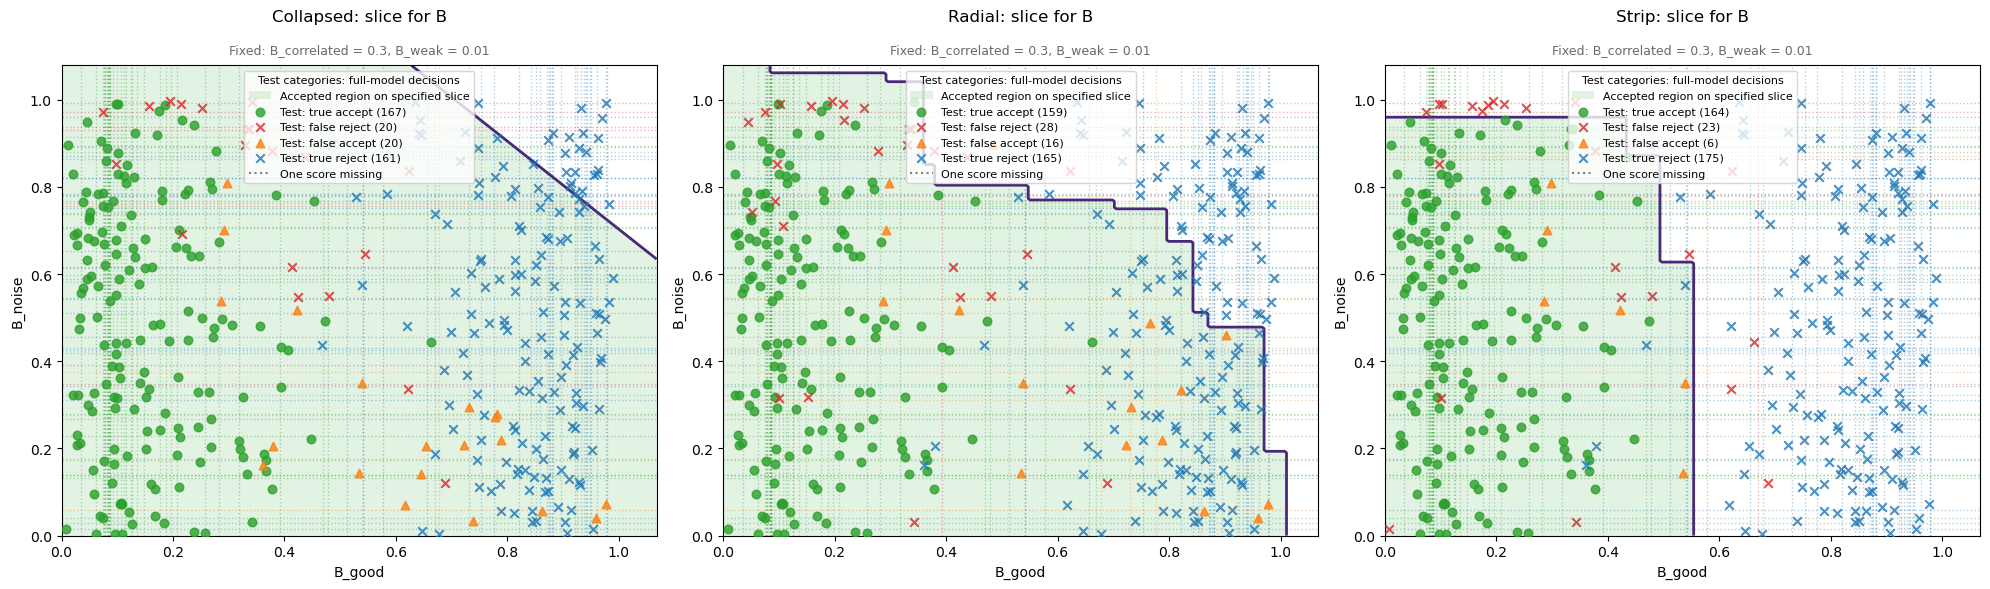
\includegraphics[width=\linewidth]{Plots/2d_envelope_synthetic.png}
\caption{Envelopes of the three constructions. The two dimensional envelope of one class of the 
simulated data, fitted on two predictors only. The shaded region is the accepted region, and the 
markers show test samples accepted or rejected by this two dimensional envelope.}
\label{fig:envelopes}
\end{figure}

\paragraph{Properties and missing scores.} The three scaling functions share one structural property.

\begin{proposition}\label{prop:monotone}
Fix an observed set $m$ and let $v,v'$ be score vectors with observed set $m$ such that $v'_j\le v_j$ for all $j\in m$. Then 
$\tau(v',m)\le\tau(v,m)$ for each of the three constructions. In particular, every accepted region $\{\tau\le\hat t\}$ is downward 
closed, so if a candidate class is accepted, it stays accepted when its scores improve.
\end{proposition}

\begin{proof}
For \eqref{eq:collapsed} this is clear, because $\tilde q$ does not depend on $v$ and the mean is nondecreasing in each coordinate. 
In \eqref{eq:radial} each ratio $v_j/(b_{pj}+\varepsilon)$ is nondecreasing in $v_j$, and a maximum and a minimum of nondecreasing 
functions is nondecreasing. For \eqref{eq:strip}, $v'_j\le v_j$ gives $\beta_j(v'_j)\le\beta_j(v_j)$ because $\beta_j$ is 
nondecreasing, so $L_{j,i,\beta_j(v'_j)} \ge L_{j,i,\beta_j(v_j)}$ by \eqref{eq:monotone}. Together with $v'_i\le v_i$, every ratio 
in \eqref{eq:strip} gets smaller. The case $|m|=1$ is again a ratio that is nondecreasing in $v_j$.
\end{proof}

The proposition is not needed for the coverage statement of Section~\ref{sec:setup}. For fixed $S_1$ (and fixed directions $u_r$, 
which are drawn independently of $S_2$ and of the new observation), each $\tau$ is a fixed function of $(v,m)$, so the same rank 
argument applies to all three. Monotonicity is only a sanity property of the learned shapes.

For a vector with observed set $m$, the collapsed method averages over $m$, and the radial and strip methods only use the 
coordinates in $m$. If no coordinate is observed, the collapsed method rejects the candidate class, while the radial and strip 
methods accept it. During fitting we require every vector in $S_1$ and $S_2$ to have at least one observed coordinate, so the 
calibration does not cover this case and we make no coverage claim for it.
% \section{Software}\label{sec:software}

The constructions of Section~\ref{sec3:constructions} are implemented in the Python package 
\texttt{conformal\_envelopes}~\citep{conformalenvelopes}. It depends only on NumPy, pandas and Matplotlib, and it is 
installed from the repository with \texttt{pip install -e .}. The package does not train any classifier. It takes the 
scores of predictors that were trained on separate data beforehand (as required in Section~\ref{sec:setup}).

% \paragraph{Input.} 
The data are a table (a pandas data frame or a CSV file) with one row per sample, an identifier column, 
a label column (needed only for fitting) and one column for each score. By default the scores lie in $[0,1]$; a higher 
score means better agreement with the class, and a missing score is NaN. The library converts the scores to the 
nonconformity scores $v=1-s$ of Section~\ref{sec:setup}. All classes use the same score columns by default. If the 
predictors give a separate score for each candidate class, as in the example below, a dictionary \texttt{label\_to\_columns} 
lists the columns of each class.


We illustrate the usage on the Iris data, using two classifiers trained on a separate part of the data, which give one 
score for each species, and the radial envelope is fitted on a conformal sample. The notebook in the repository contains 
the same steps, with additional checks and plots.


{\footnotesize
\begin{verbatim}
import pandas as pd
from sklearn.datasets import load_iris
from sklearn.linear_model import LogisticRegression
from sklearn.neighbors import KNeighborsClassifier
from sklearn.model_selection import train_test_split
from conformal_envelopes import ConformalSetModel, evaluate_prediction_sets

iris = load_iris(as_frame=True)
X, y = iris.data, iris.target_names[iris.target]
X_rest, X_test, y_rest, y_test = train_test_split(
    X, y, test_size=30, stratify=y, random_state=0)
X_train, X_cal, y_train, y_cal = train_test_split(
    X_rest, y_rest, test_size=60, stratify=y_rest, random_state=1)

# Two classifiers give one score per candidate species.
clfs = {"logreg": LogisticRegression(max_iter=2000),
        "knn": KNeighborsClassifier()}
for clf in clfs.values():
    clf.fit(X_train, y_train)

def score_table(features):
    table = pd.DataFrame({"ID": features.index.astype(str)})
    for name, clf in clfs.items():
        for k, species in enumerate(clf.classes_):
            table[f"{species}_{name}"] = clf.predict_proba(features)[:, k]
    return table

cal = score_table(X_cal)
cal["label"] = y_cal
test = score_table(X_test)
cols = {s: [f"{s}_logreg", f"{s}_knn"] for s in iris.target_names}

model = ConformalSetModel(method="radial", alpha=0.10, random_state=0)
model.fit(cal, id_col="ID", label_col="label",
          score_cols=[c for v in cols.values() for c in v],
          label_to_columns=cols)
pred = model.predict(test)
print(evaluate_prediction_sets(pred["prediction_set"], list(y_test)))
\end{verbatim}
}


The model is created with the method (\texttt{"collapsed"}, \texttt{"radial"} or \texttt{"strip"}), the level $\alpha$ and 
the optional parameters of the method from Section~\ref{sec3:constructions}. \texttt{fit} splits the sample of each class 
into $S_1$ and $S_2$ (a fraction \texttt{shape\_fraction}, $0.5$ by default, goes to $S_1$), builds the envelope and 
computes $\hat t$. \texttt{predict} returns one row for each sample, with the prediction set, its size, the value of $\tau$ 
for each label and an indicator \texttt{forced}. The optional rule that replaces an empty set by the label with the smallest 
$\tau$ is on by default (\texttt{force\_nonempty}), and it is switched off in Section~\ref{sec:experiments}. 
\texttt{evaluate\_prediction\_sets} computes the coverage, the average set size, the singleton rate, the empty set rate and 
the coverage of each class. Finally, a fitted model can be saved and loaded.

\paragraph{Visualisation.} \texttt{plot} fits a separate two dimensional envelope for two selected predictors and shows it 
with the test samples, as in Figure~\ref{fig:envelopes}. \texttt{plot\_slice} shows a cross section of the fitted envelope, 
with the other coordinates fixed at chosen values. Finally, for each true class \texttt{plot\_inclusion\_heatmap} shows 
how often every label appears in the prediction sets, and its diagonal gives the coverage of each class.

\paragraph{Examples} The repository contains notebooks for the Iris tutorial above, the simulated experiment 
and the two football experiments of Section~\ref{sec:experiments}. Since $30$ test flowers are too few to judge the 
coverage, the Iris example only illustrates the use of the library. 
% \section{Experiments}\label{sec:experiments}

We evaluated the three envelope construction methods on simulated data with missing scores and on two football 
classification tasks. We use $\alpha=0.1$ throughout, and the sample of each class is split equally into the shape discovery 
set $S_1$ and the size scaling set $S_2$. The coverage is the proportion of test samples whose prediction set contains 
the true label. We report coverage, the average set size, the singleton rate and the empty-set rate, as mean $\pm$ 
standard error over repeated runs. The radial method uses $M=100$, $\kappa=4$ and $\delta=30^\circ$, and the strip 
method uses $NB=8$ with $n_0=3$ on the simulated data and $n_0=10$ on the football data; all other parameters are the 
default parameters in the library. The code and the saved outputs are available at \citep{conformalenvelopes}.
% \url{https://github.com/Nizalia13/Conformal_Classification_Library}.

\paragraph{Simulated data.} There are two classes, $A$ and $B$, and four predictors which are used to score each candidate 
class. For a sample with true class $h^\ast$ and a candidate class $h$, let $\sigma=+1$ if $h=h^\ast$ and $\sigma=-1$ 
otherwise. The first predictor has the score $1/(1+e^{-(1.8\,\sigma+\varepsilon_1)})$ with $\varepsilon_1\sim N(0,1)$. 
The second is built in the same way from a noise term $\varepsilon_2$ with correlation $0.9$ to $\varepsilon_1$. The 
third is weak, it has a shift $0.35\,\sigma$ and noise of standard deviation $1.5$, and the fourth is uniform on $[0,1]$, 
it carries no information. Each score is then independently hidden with probability $0.15$. If all four scores of a 
candidate are hidden the draw is repeated. In each run there are $1500$ training draws and $500$ test samples, and we use 
$500$ independent runs.

\paragraph{Football data.} We classify FIFA~19 players from $34$ skill ratings \citep{fifa19data}. In the first task 
the label is simpler, it is just the role (defender, midfielder, attacker or goalkeeper) for $18{,}147$ players. In the 
second it is the recorded position, in this we only use the $17{,}835$ players in the $20$ positions with at least $100$ 
player records. Four classifiers (logistic regression, random forest, gradient boosting and a support vector classifier) 
are trained on a separate $40\%$ of the players, and the scores are their predicted probabilities of each label. Another
$20\%$ is used for validation, and the remaining players are used for conformal fitting ($30\%$) and testing ($10\%$). 
To measure the variability of the coverage, we keep the trained classifiers fixed and evaluate them over $100$ random splits 
of the remaining data into calibration and test sets (sized $5{,}444$ / $1{,}815$ for roles and 
$5{,}351$ / $1{,}784$ for positions). The data contain no missing scores.

 
\begin{table}[ht]
\centering
\small
\begin{tabular}{llcccc}
\toprule
Data & Method & Coverage & Set size & Singleton & Empty \\
\midrule
Simulated & Collapsed & $0.9012\pm0.0008$ & $1.014$ & $0.811$ & $0.088$ \\
($500$ runs) & Radial & $0.9001\pm0.0008$ & $1.086$ & $0.752$ & $0.081$ \\
 & Strip & $0.8998\pm0.0008$ & $0.955$ & $0.856$ & $0.095$ \\
\midrule
Football roles & Collapsed & $0.9002\pm0.0009$ & $1.069$ & $0.887$ & $0.022$ \\
($100$ runs) & Radial & $0.8995\pm0.0010$ & $1.068$ & $0.886$ & $0.023$ \\
 & Strip & $0.8994\pm0.0010$ & $1.082$ & $0.856$ & $0.031$ \\
\midrule
Football positions & Collapsed & $0.9032\pm0.0009$ & $4.364$ & $0.108$ & $0.010$ \\
($100$ runs) & Radial & $0.9016\pm0.0009$ & $4.738$ & $0.101$ & $0.010$ \\
 & Strip & $0.9016\pm0.0009$ & $4.575$ & $0.118$ & $0.011$ \\
\bottomrule
\end{tabular}
\caption{Results as mean $\pm$ standard error over repeated runs, with target coverage $0.9$.}
\label{tab:results}
\end{table}

\paragraph{Results.} Table~\ref{tab:results} shows that the coverage of all three constructions is close to the target 
$0.9$ in every experiment. The coverage of each class is also close to the target; it is between $0.899$ and $0.902$  on 
the simulated data, and between $0.896$ and $0.902$  for the four roles. For the positions, the average coverage of a 
position lies between $0.888$ and $0.926$, it has more range due to the smaller number of data points for each position.

The methods have similar set sizes on the football role tasks, where most of the sets are singletons. But on the position 
classification task the sets contain between $4.4$ and $4.7$ positions on average, which is expected, because neighbouring 
positions, such as the left, central and right variants of a role, have very similar skill values. The order of the methods 
by set size changes between the experiments, therefore we cannot claim that one construction is better in general. The 
football dataset is complete, so the handling of missing scores is only evaluated on the simulated data.
% \section{Discussion and limitations}\label{sec:discussion}

We presented three class specific conformal envelopes for classification with several predictors: a collapsed, a radial 
and a strip envelope. They share the same two stage calibration procedure and the same coverage statement, they use only the 
observed scores of a sample, and they are implemented in an open source Python package. In our experiments the coverage 
of all three constructions was close to the nominal level, and none of them was better than the others in every experiment.

The coverage statement of Section~\ref{sec:setup} has limits. It holds for each class and not conditionally on the input 
$x$, and it assumes that the samples of a class are exchangeable and that the missingness of the scores has the same 
distribution in the calibration and in the test data. Filtering the candidate classes before the prediction can make it 
fail whenever the filter removes the true class. If a class has few calibration samples, its threshold is infinite and 
its envelope accepts every sample, which gives large prediction sets. 

The experiments also have limits. The simulated data come from one generator in which scores are hidden completely at 
random, and the football data have no missing scores, so we did not study scores that are missing for a reason related 
to the class. We compared the three constructions only with each other, with the collapsed envelope as the simplest 
baseline. We did not compare them with other conformal methods that combine several predictors, in particular the method 
of \citet{ochoarivera2024conformal}. The parameters of the radial and strip envelopes were set to defaults and were not 
tuned. Comparisons with these methods, scores that are not missing at random, and tuning of the parameters are directions 
for future work.

% \printcredits

% \section*{Declaration of generative AI and AI-assisted technologies in the manuscript preparation process}
% During the preparation of this work the author(s) used ChatGPT (OpenAI) and Claude (Anthropic) to review the code, to check the mathematical statements against the code, to write scripts for the repeated experiments, and to draft and edit parts of the text. After using these tools, the author(s) reviewed and edited the content as needed and take(s) full responsibility for the content of the published article.

% \section*{Data and code availability}
% The code of the package and of all experiments is available at \url{https://github.com/Nizalia13/Conformal_Classification_Library}. The simulated data are generated by the code. The football data are public \citep{fifa19data}.

% \section*{Funding}
% This research did not receive any specific grant from funding agencies in the public, commercial, or not-for-profit sectors.

% % \section*{Acknowledgements}
% % To be written.

% \bibliographystyle{cas-model2-names}
% \bibliography{references}

% \end{document}



\documentclass[a4paper,fleqn]{cas-sc}
\usepackage[authoryear,longnamesfirst]{natbib}
\usepackage{amsmath,amssymb}
\usepackage{graphicx}
\usepackage{url}
\usepackage{float}

\newtheorem{theorem}{Theorem}
\newtheorem{proposition}[theorem]{Proposition}
\newproof{proof}{Proof}



\begin{document}
\let\WriteBookmarks\relax
\def\floatpagepagefraction{1}
\def\textpagefraction{.001}

\shorttitle{Conformal envelopes}
\shortauthors{Nizalia Siddiqui \& Clovis Galiez}

\title[mode=title]{Conformal envelopes: class specific conformal prediction sets with missing scores}

\author[1]{Nizalia Siddiqui}
\cormark[1]
\fnmark[1]
\ead{nizaliasiddiqui25@gmail.com}
% \credit{Methodology, Software, Validation, Formal analysis, Investigation, Writing -- original draft}
\credit{Methodology, Software, Validation, Experimentation, Writing}

\author[1]{Clovis Galiez}
\ead{clovis.galiez@univ-grenoble-alpes.fr}
% \credit{Conceptualization, Methodology, Supervision, Writing -- review and editing}
\credit{Conceptualization, Methodology, Supervision, Writing}

\affiliation[1]{organization={Univ. Grenoble Alpes, CNRS, Grenoble INP, LJK},
            addressline={150 Place du Torrent, Campus Universitaire Saint-Martin-d'H\`eres},
            postcode={38401},
            city={Grenoble},
            country={France}}

\cortext[1]{Corresponding author}
\fntext[1]{Present address: Islamabad, Pakistan}

%%%%%%%%%%%%%%%%%%%%%%%%%%%%%%%%%%%%%%%%%%%%%%%%%%%%%%%%%%%%%%%%%%%%%%%%%%%%%%%%%%%%%%%%%%%

\begin{abstract}
Conformal prediction uses the output of a trained predictor and returns a prediction set that contains the true label 
with a chosen probability. When there are several predictors scoring each candidate class, the scores have to be 
combined, and the way they are combined influences the size of the sets. We present class specific conformal envelopes 
for classification. For each class, the shape of an envelope in the space of the score vectors is learned on one part of 
the calibration data of that class, and its size is scaled on the other part. Here we propose three envelope construction 
methods: a collapsed envelope that averages the scores, a radial envelope whose boundary depends on the direction of the 
score vector, and a strip envelope that bounds each score given the value of another score. All three methods only use 
the observed scores of a sample, so samples with missing scores still receive prediction sets. We show that when the 
samples of a class are exchangeable and the missingness has the same distribution in the calibration and test data, the 
sets have at least the nominal level of class conditional coverage. These constructions are implemented in an open source 
Python package. In experiments on simulated data with missing scores and on football player classification with four 
roles and with twenty positions, the average coverage of all three constructions is between 0.899 and 0.903 for a 
target of 0.9, the set sizes are similar, and no construction is best in every experiment.

\end{abstract}

\begin{highlights}
\item Class specific conformal envelopes built from scores from several predictors
\item Three envelope construction methods (collapsed, radial, strip)
\item Class conditional coverage guarantee within each class under exchangeability
\item Samples with missing scores still receive prediction sets
\item Open source Python package; coverage near 90\% on simulated and football data
\end{highlights}

\begin{keywords}
conformal prediction \sep classification \sep missing scores \sep prediction sets \sep software
\end{keywords}

\maketitle

\section{Introduction}\label{sec:intro}

Conformal prediction can be used to turn the output of any trained predictor into a prediction set that contains the 
true label with a defined probability, and it needs no assumption on the distribution of the data except exchangeability 
\citep{vovk2005algorithmic,shafer2008tutorial,angelopoulos2023conformal}. In classification, the set is built from a 
nonconformity score, which measures how badly a candidate label agrees with an input. The coverage guarantee holds 
for every choice of score, but the choice affects the size of the sets. A poorly chosen score gives sets that are valid 
but too large to be useful.

Several predictors also often score each candidate class, for example classifiers with different models or different input 
features. These candidate scores are then combined into a vector, which is aggregated into a single scalar score. A 
fixed rule such as the mean treats all predictors in the same way, even though they can differ in reliability and they 
can be dependent on other predictors. Mostly the methods for conformal aggregation combine the prediction sets of the 
individual predictors \citep{gasparin2024merging,yang2024selection}, or project the score vector on one weighted direction 
\citep{luo2024weighted}. Instead of this, \citet{ochoarivera2024conformal} work in score space. They 
define a quantile envelope for the multivariate score as the intersection of half spaces along random directions, learn 
its shape on one part of the calibration data and scale it on the other part, which gives marginal coverage.

In this paper we build on this idea in a classification setting. The envelope is learned separately for each class, 
from the score vectors of the samples of that class, so that the coverage statement holds for each class. This is known 
as Mondrian conformal prediction \citep{vovk2005algorithmic}. We present three envelope constructions that share the same 
two stage calibration: a collapsed envelope, which averages the scores, a radial envelope, in which the boundary changes 
with the direction of the score vector, and a strip envelope, which bounds each coordinate given the value of another 
coordinate. The radial and strip envelopes are not intersections of half  spaces, and all three constructions use only 
the observed scores of a sample, so a score vector with missing entries can still be assigned a prediction set.


Our contributions are the radial and strip constructions, the handling of missing scores, an open source Python package that 
implements them (Section~\ref{sec:software}), and experiments on simulated data with missing scores and on football player 
data (Section~\ref{sec:experiments}). In these experiments the coverage is close to the nominal level for all three 
constructions, and we do not claim that one of them is better than the others in general. The last section discusses the 
limitations of our work.

\section{Setup and calibration}\label{sec:setup}

Let $\mathcal H=\{h_1,\dots,h_N\}$ be the discrete set of candidate classes. Our aim is to build a function $C$ that maps an 
input $x$ to a subset $C(x)\subseteq\mathcal H$ of classes, such that the true class lies in the set with probability at least 
$1-\alpha$. Our input is described by scores from several predictors. For each candidate class $h$ we have a raw score vector 
$s_h=(s_{h,1},\dots,s_{h,K_h})\in([0,1]\cup\{\mathrm{NA}\})^{K_h}$, where $s_{h,k}$ is the evidence of the $k$-th predictor in 
favour of class $h$, while $\mathrm{NA}$ means that this predictor gave no score for the given class. We do not impute missing 
scores $(\mathrm{NA})$. Instead, we record the set of observed coordinates $m_h=\{k:s_{h,k}\neq\mathrm{NA}\}$ and define all 
scoring functions on the pairs $(s_h,m_h)$ and not on $s_h$ alone. A score close to $1$ means strong evidence for $h$, thus we 
map every observed coordinate to the nonconformity score $v_{h,k}=1-s_{h,k}$. When $h$ is the true class, the vector $v_h$ 
concentrates near the origin, while if $h$ is not the true class, the vector $v_h$ is further away. In 
Section~\ref{sec3:constructions} we write $v$ for such a vector $v_h$ and drop the index $h$.

Suppose we have a labelled calibration sample $\{(x_i,y_i)\}$. The predictors that produce the scores are trained on data that 
is disjoint from this sample and the test points. For each class $h$, the points with $y_i=h$ are randomly split into the shape  
discovery set $S_{1,h}$ and the size scaling set $S_{2,h}$. Each pair $(v_h(x_i),m_h(x_i))$ shows the score pattern for class 
$h$ when it is actually the true class. A separate envelope is fitted for every class, using only the samples of that class.

Using $S_{1,h}$, we construct the scalar score $\tau_h(v,m)$, using one of the three envelope construction techniques in 
Section~\ref{sec3:constructions}. We then compute the class specific scale factor $\hat t_h$ on $S_{2,h}$ as:
\begin{equation}\label{eq:qhat}
\hat t_h=\tau_{h,(k_h)},\qquad k_h=\lceil(|S_{2,h}|+1)(1-\alpha)\rceil,
\end{equation}

where $\tau_{h,(k)}$ is the $k$-th smallest value of $\{\tau_h(v,m):(v,m)\in S_{2,h}\}$, and $\hat t_h=\infty$ if 
$k_h>|S_{2,h}|$. The threshold value $\hat t_h$ is can be computed directly since the calibration set of class $h$ only contains 
samples of this class. The prediction set of a new input $x$ contains every class whose scaled envelope accepts the scores of $x$,
\begin{equation}\label{eq:set}
C(x)=\bigl\{h\in\mathcal H:\ \tau_h\bigl(v_h(x),m_h(x)\bigr)\le\hat t_h\bigr\}.
\end{equation}

\begin{theorem}[Class-conditional coverage]\label{thm:coverage}
Assume that for every class $h$, the pairs $(v_h,m_h)$ of the samples in $S_{1,h}$ and $S_{2,h}$ and of a new sample with true 
class $h$ are exchangeable. Then, for every $h\in\mathcal H$,
\[ \mathbb P\bigl(Y\in C(X)\mid Y=h\bigr)\ \ge\ 1-\alpha ,\]
and in particular $\mathbb P(Y\in C(X))\ge 1-\alpha$. If in addition the values of $\tau_h$ are almost surely distinct, then 
$\mathbb P(Y\in C(X)\mid Y=h)\le 1-\alpha+1/(|S_{2,h}|+1)$.
\end{theorem}

\begin{proof}
Let us fix a class $h$ and write $n=|S_{2,h}|$ and $k=k_h$. We condition on $S_{1,h}$ and on the random directions of the radial 
method, which are independent of $S_{2,h}$ and of the new sample. Then $\tau_h$ is a fixed function. Let $T_1,\dots,T_n$ be its 
values on $S_{2,h}$ and let $T_0$ be its value on a new sample with $Y=h$. Since $T_0, \dots, T_n$ are exchangeable, the rank of 
$T_0$ is uniformly distributed over $\{1, \dots, n+1\}$ when there are no ties, and ties can only make the rank of $T_0$ smaller. 
The event $\{h\in C(X)\}$ is $\{T_0\le T_{(k)}\}$, so  \[ \mathbb P\bigl(T_0\le T_{(k)}\bigr)\ \ge\ \frac{k}{n+1}\ \ge\ 1-\alpha .\]
If $k>n$ then $\hat t_h=\infty$ and the probability is $1$. If the values are almost surely distinct, the probability equals 
$k/(n+1)<1-\alpha+1/(n+1)$. Averaging over $S_{1,h}$ and the directions gives the class conditional statement, and averaging over 
$h$ with the class probabilities gives the marginal one.
\end{proof}

This is the Mondrian form of conformal prediction \citep{vovk2005algorithmic}. It does not give coverage conditional on an 
individual input $x$, which is not possible in finite samples without strong assumptions. The observed sets $m_h$ are part of the 
exchangeable pairs, so a new sample must have the same missingness mechanism as the calibration samples. If a class has few 
calibration samples, so that $k_h>|S_{2,h}|$, its threshold is infinite and it is always accepted. The library can also return 
the class with the smallest normalized score $\tau_h/\hat t_h$ when $C(x)$ is empty. This only enlarges the set, so the lower 
bound still holds, but we do not use this option in our experiments, which means that empty sets count as errors.

\section{Envelope constructions}
\label{sec3:constructions}

Each of the three envelope construction methods follows the same two stage calibration procedure: the shape-discovery set $S_1$ is 
used to determine the geometric shape of the envelope, then the size scaling set $S_2$ is used to determine the scaling factor 
$\hat t$. Each construction assigns a scalar score, $\tau(v,m)$, to a score vector $v$ with observed set $m$. A candidate class is 
then included in the prediction set when $\tau(v,m)\le\hat t$, where $\hat t$ is calculated on $S_2$ as in Section~\ref{sec:setup}. 
For both the collapsed and radial methods, we define $\tau(v)=\inf\{t>0: v\in t\cdot E\}$ using an envelope $E$ which is star shaped 
with respect to the origin and give a closed form expression for it. The strip method works in the same way, except that the 
single scaling factor $\hat t$ multiplies the limits of the staircase rather than dilating the whole region, so $\tau$ is defined 
directly as a maximum of ratios.

We first fix a class $h$ and drop the index $h$. $K$ denotes the number of coordinates that remain after removing the coordinates 
that are missing for every sample of $S_1$. For a vector $v\in[0,\infty)^K$ and observed set $m\subseteq\{1,\dots,K\}$, we write 
$v_j$, $j\in m$, for just its observed entries. We use $\varepsilon=10^{-12}$ to prevent division by zero, and $Q_p(\cdot)$ denotes 
the empirical $p$-quantile.


%%%%%%%%%%%%%%%%%%%%%%%%%%%%%%%%%%%%%%%%%%%%%%%%%%%%%%%%%%%%%%%%%%%%%%%%%%%%%%%%%%%%%%%%%%%%%%%%%%%%%%%%%%%%%%%%%%%%%%%%%%%%%%%
\paragraph{Collapsed envelope.} The basic envelope construction simply collapses the $K$-dimensional score vector to a scalar score 
by taking the mean over the observed coordinates, and calibrates a single quantile on $S_1$:
\begin{equation}\label{eq:collapsed}
\bar v=\frac{1}{|m|}\sum_{j\in m}v_j,\qquad \tilde q=Q_{1-\alpha}\bigl(\{\bar v:v\in S_1\}\bigr),\qquad
\tau(v,m)=\frac{\bar v}{\tilde q},\qquad
E=\{v:\bar v\le\tilde q\}.
\end{equation}

This method discards the geometric information that the $K$ coordinates provide. Two vectors with the same mean are treated 
identically whatever the distribution of their coordinates is, so a single coordinate with strong evidence (a very small $v_j$) is 
averaged together with all the others. The accepted region is a halfspace in the observed coordinates. It serves as a mean score baseline 
for the multidimensional constructions below. After calibration on $S_2$, a vector is accepted when $\bar v/\tilde q\le\hat t$, 
which is the same as $\bar v\le\hat t\,\tilde q$. Here $\hat t$ is the $k$-th smallest value of $\bar v/\tilde q$ over $v\in S_2$, 
so $\hat t\,\tilde q$ is just the $k$-th smallest value of of $\bar v$ over $v\in S_2$. 
% This means that $\tilde q$ does not change the prediction set, and for this method $S_1$ is only 
% used to decide which coordinates are kept.



%%%%%%%%%%%%%%%%%%%%%%%%%%%%%%%%%%%%%%%%%%%%%%%%%%%%%%%%%%%%%%%%%%%%%%%%%%%%%%%%%%%%%%%%%%%%%%%%%%%%%%%%%%%%%%%%%%%%%%%%%%%%%%%
 
\paragraph{Radial envelope.} The radial envelope method retains the directional information of the scores. It works by calibrating 
a boundary radius as a function of direction on the unit sphere, which is restricted to the positive orthant since all nonconformity 
scores are nonnegative. We sample $M$ directions $\{u_r\}_{r=1}^M$ uniformly from the positive orthant by drawing independent vectors $g_r\sim|\mathcal 
N(0,I_K)|$ and normalizing them, $u_r=g_r/\|g_r\|$. For each vector $v\in S_1$, we compute its norm $\Vert{}v\Vert{}$ and  
unit direction $d_v = v / \Vert{}v\Vert{}$ using only the observed coordinates.
For each direction $u_r$, we collect the $n_r$ points of $S_1$ within an angular sector of half width $\delta=30^\circ$, that is, 
those with $d_v\cdot u_r\ge\cos\delta$. The directional radius $\tilde q_r$ is then calibrated as
\begin{equation}\label{eq:radii}
\tilde q_r=\begin{cases}
Q_{1-\alpha}\bigl(\{\|v\|:d_v\cdot u_r\ge\cos\delta\}\bigr) & \text{if } n_r\ge n_{\min},\\[1ex]
w_r\,Q_{1-\alpha}\bigl(\{\|v\|:d_v\cdot u_r\ge\cos\delta\}\bigr)+(1-w_r)\,\tilde q_{\mathrm{marg}} & \text{if } 
0<n_r<n_{\min},\\[1ex]
\tilde q_{\mathrm{marg}} & \text{if } n_r=0,
\end{cases}
\end{equation}

where $n_{\min}=\max\{10,\lfloor 0.2\,|S_1|\rfloor\}$ is the minimum number of points required, $w_r=n_r/n_{\min}$, and 
$\tilde q_{\mathrm{marg}}=Q_{1-\alpha}(\{\|s\|:s\in S_1\})$ is the marginal fallback radius. This helps us avoid a hard 
cutoff between sufficient and insufficient local support. To get a smooth boundary, we compute the radius in an arbitrary direction 
$d$ as a weighted average of all $M$ calibrated radii,
\begin{equation}\label{eq:smooth}
R(d)=\sum_{r=1}^{M}\omega_r(d)\,\tilde q_r,\qquad
\omega_r(d)=\frac{\exp(\kappa\,d\cdot u_r)}{\sum_{r'=1}^{M}\exp(\kappa\,d\cdot u_{r'})},
\end{equation}
where $\kappa>0$ controls the angular smoothness (a larger $\kappa$ gets closer to nearest-direction assignment). We evaluate $R$ 
at the directions $a_p\in\{u_1,\dots,u_M,e_1,\dots,e_K\}$, where the $e_j$ are the coordinate axes. This gives us the boundary points 
$b_p=R(a_p)\,a_p$. The envelope $E$ is the union of the boxes $\{v:0\le v\le b_p\}$ over all $p$, and the scaling function has the 
closed form:
\begin{equation}\label{eq:radial}
\tau(v,m)=\min_{p}\;\max_{j\in m}\;\frac{v_j}{b_{pj}+\varepsilon},
\end{equation}
which is $\inf\{t>0:v\in t\cdot E\}$ computed on the observed coordinates. We use $M=250$ and $\kappa=8$ by default.

%%%%%%%%%%%%%%%%%%%%%%%%%%%%%%%%%%%%%%%%%%%%%%%%%%%%%%%%%%%%%%%%%%%%%%%%%%%%%%%%%%%%%%%%%%%%%%%%%%%%%%%%%%%%%%%%%%%%%%%%%%%%%%%

%  → 
%  →  (twice, in the limits equation)

\paragraph{Strip envelope.} The strip envelope works by defining conditional bounds for each target coordinate $i$ based on the 
bin occupied by another coordinate $j$. We partition the range of the observed $S_1$ values of coordinate $j$ into $NB$ equal width 
bins, and write $\beta_j(x)$ for the bin that contains $x$ (a value below the smallest or above the largest observed $S_1$ value of 
coordinate $j$ is put in the first or last bin, respectively). We work with the level $\alpha'=\alpha/K$, a Bonferroni type correction 
for the $K$ coordinates. It only affects the shape of the envelope, since the coverage is controlled by $\hat t$. For each bin $n$ 
containing $n_{j,n}$ points of $S_1$ with both $v_j$ and $v_i$ observed, the upper limit along coordinate $i\neq j$ is calibrated as
\begin{equation}\label{eq:limits}
L_{j,i,n}=\begin{cases}
Q_{1-\alpha'}\bigl(\{v_i:v\in S_1,\ \beta_j(v_j)=n\}\bigr) & \text{if } n_{j,n}\ge n_0,\\[1ex]
w_{j,n}\,Q_{1-\alpha'}\bigl(\{v_i:v\in S_1,\ \beta_j(v_j)=n\}\bigr)+(1-w_{j,n})\,\tilde q_i & \text{if } 0<n_{j,n}<n_0,\\[1ex]
\tilde q_i & \text{if } n_{j,n}=0,
\end{cases}
\end{equation}
where $\tilde q_i$ is the marginal $(1-\alpha')$ quantile of coordinate $i$ over $S_1$, $n_0$ is the minimum number of points required 
in a bin, and $w_{j,n}=n_{j,n}/n_0$ shrinks the limit of underpopulated bins towards it, which is similar to the blending rule of the 
radial envelope. Then there is a monotonicity pass that makes sure that the limits are nonincreasing in the bin index,
\begin{equation}\label{eq:monotone}
L_{j,i,n}\leftarrow\max_{n'\ge n}L_{j,i,n'}.
\end{equation}
This ensures that a vector with a smaller value (more confident) in the conditioning coordinate $j$ never receives a tighter bound 
on coordinate $i$ than a vector with a larger value in $j$. The envelope $E$ is a coordinatewise monotone staircase, which is the intersection of these 
pairwise constraints. If a coordinate is unobserved, we ignore all the pairwise constraints involving it, so it is neither used as 
a target nor as a conditioning coordinate. The scaling function is
\begin{equation}\label{eq:strip}
\tau(v,m)=\begin{cases}
\displaystyle\max_{\substack{j,i\in m\\ j\ne i}}\ \dfrac{v_i}{L_{j,i,\beta_j(v_j)}+\varepsilon}, & |m|\ge 2,\\[3ex]
\dfrac{v_j}{\tilde q_j+\varepsilon}, & m=\{j\},
\end{cases}
\end{equation}
so a vector is accepted when $v_i\le\hat t\,L_{j,i,\beta_j(v_j)}$ for every pair of observed coordinates. The single scalar 
$\hat t$ multiplies all the limits, while the bins stay fixed. We use $NB=8$ and $n_0=3$ by default. Figure~\ref{fig:envelopes} 
shows the three envelopes for two predictors.

%%%%%%%%%%%%%%%%%%%%%%%%%%%%%%%%%%%%%%%%%%%%%%%%%%%%%%%%%%%%%%%%%%%%%%%%%%%%%%%%%%%%%%%%%%%%%%%%%%%%%%%%%%%%%%%%%%%%%%%%%%%%%%%
\begin{figure}[H]
\centering
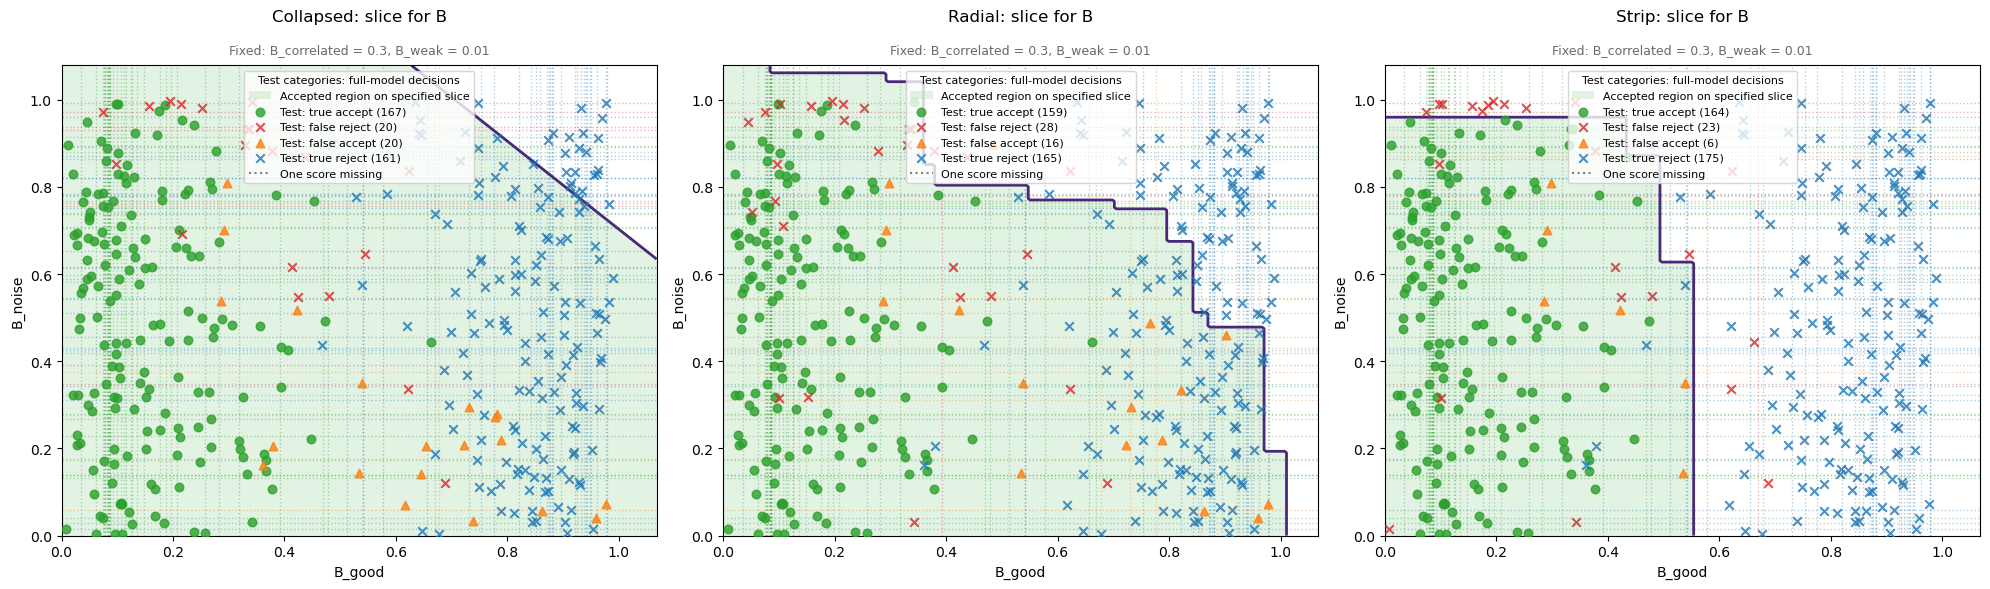
\includegraphics[width=\linewidth]{Plots/2d_envelope_synthetic.png}
\caption{Envelopes of the three constructions. The two dimensional envelope of one class of the 
simulated data, fitted on two predictors only. The shaded region is the accepted region, and the 
markers show test samples accepted or rejected by this two dimensional envelope.}
\label{fig:envelopes}
\end{figure}

\paragraph{Properties and missing scores.} The three scaling functions share one structural property.

\begin{proposition}\label{prop:monotone}
Fix an observed set $m$ and let $v,v'$ be score vectors with observed set $m$ such that $v'_j\le v_j$ for all $j\in m$. Then 
$\tau(v',m)\le\tau(v,m)$ for each of the three constructions. In particular, every accepted region $\{\tau\le\hat t\}$ is downward 
closed, so if a candidate class is accepted, it stays accepted when its scores improve.
\end{proposition}

\begin{proof}
For \eqref{eq:collapsed} this is clear, because $\tilde q$ does not depend on $v$ and the mean is nondecreasing in each coordinate. 
In \eqref{eq:radial} each ratio $v_j/(b_{pj}+\varepsilon)$ is nondecreasing in $v_j$, and a maximum and a minimum of nondecreasing 
functions is nondecreasing. For \eqref{eq:strip}, $v'_j\le v_j$ gives $\beta_j(v'_j)\le\beta_j(v_j)$ because $\beta_j$ is 
nondecreasing, so $L_{j,i,\beta_j(v'_j)} \ge L_{j,i,\beta_j(v_j)}$ by \eqref{eq:monotone}. Together with $v'_i\le v_i$, every ratio 
in \eqref{eq:strip} gets smaller. The case $|m|=1$ is again a ratio that is nondecreasing in $v_j$.
\end{proof}

The proposition is not needed for the coverage statement of Section~\ref{sec:setup}. For fixed $S_1$ (and fixed directions $u_r$, 
which are drawn independently of $S_2$ and of the new observation), each $\tau$ is a fixed function of $(v,m)$, so the same rank 
argument applies to all three. Monotonicity is only a sanity property of the learned shapes.

For a vector with observed set $m$, the collapsed method averages over $m$, and the radial and strip methods only use the 
coordinates in $m$. If no coordinate is observed, the collapsed method rejects the candidate class, while the radial and strip 
methods accept it. During fitting we require every vector in $S_1$ and $S_2$ to have at least one observed coordinate, so the 
calibration does not cover this case and we make no coverage claim for it.
\section{Software}\label{sec:software}

The constructions of Section~\ref{sec3:constructions} are implemented in the Python package 
\texttt{conformal\_envelopes}~\citep{conformalenvelopes}. It depends only on NumPy, pandas and Matplotlib, and it is 
installed from the repository with \texttt{pip install -e .}. The package does not train any classifier. It takes the 
scores of predictors that were trained on separate data beforehand (as required in Section~\ref{sec:setup}).

% \paragraph{Input.} 
The data are a table (a pandas data frame or a CSV file) with one row per sample, an identifier column, 
a label column (needed only for fitting) and one column for each score. By default the scores lie in $[0,1]$; a higher 
score means better agreement with the class, and a missing score is NaN. The library converts the scores to the 
nonconformity scores $v=1-s$ of Section~\ref{sec:setup}. All classes use the same score columns by default. If the 
predictors give a separate score for each candidate class, as in the example below, a dictionary \texttt{label\_to\_columns} 
lists the columns of each class.


We illustrate the usage on the Iris data, using two classifiers trained on a separate part of the data, which give one 
score for each species, and the radial envelope is fitted on a conformal sample. The notebook in the repository contains 
the same steps, with additional checks and plots.


{\footnotesize
\begin{verbatim}
import pandas as pd
from sklearn.datasets import load_iris
from sklearn.linear_model import LogisticRegression
from sklearn.neighbors import KNeighborsClassifier
from sklearn.model_selection import train_test_split
from conformal_envelopes import ConformalSetModel, evaluate_prediction_sets

iris = load_iris(as_frame=True)
X, y = iris.data, iris.target_names[iris.target]
X_rest, X_test, y_rest, y_test = train_test_split(
    X, y, test_size=30, stratify=y, random_state=0)
X_train, X_cal, y_train, y_cal = train_test_split(
    X_rest, y_rest, test_size=60, stratify=y_rest, random_state=1)

# Two classifiers give one score per candidate species.
clfs = {"logreg": LogisticRegression(max_iter=2000),
        "knn": KNeighborsClassifier()}
for clf in clfs.values():
    clf.fit(X_train, y_train)

def score_table(features):
    table = pd.DataFrame({"ID": features.index.astype(str)})
    for name, clf in clfs.items():
        for k, species in enumerate(clf.classes_):
            table[f"{species}_{name}"] = clf.predict_proba(features)[:, k]
    return table

cal = score_table(X_cal)
cal["label"] = y_cal
test = score_table(X_test)
cols = {s: [f"{s}_logreg", f"{s}_knn"] for s in iris.target_names}

model = ConformalSetModel(method="radial", alpha=0.10, random_state=0)
model.fit(cal, id_col="ID", label_col="label",
          score_cols=[c for v in cols.values() for c in v],
          label_to_columns=cols)
pred = model.predict(test)
print(evaluate_prediction_sets(pred["prediction_set"], list(y_test)))
\end{verbatim}
}


The model is created with the method (\texttt{"collapsed"}, \texttt{"radial"} or \texttt{"strip"}), the level $\alpha$ and 
the optional parameters of the method from Section~\ref{sec3:constructions}. \texttt{fit} splits the sample of each class 
into $S_1$ and $S_2$ (a fraction \texttt{shape\_fraction}, $0.5$ by default, goes to $S_1$), builds the envelope and 
computes $\hat t$. \texttt{predict} returns one row for each sample, with the prediction set, its size, the value of $\tau$ 
for each label and an indicator \texttt{forced}. The optional rule that replaces an empty set by the label with the smallest 
$\tau$ is on by default (\texttt{force\_nonempty}), and it is switched off in Section~\ref{sec:experiments}. 
\texttt{evaluate\_prediction\_sets} computes the coverage, the average set size, the singleton rate, the empty set rate and 
the coverage of each class. Finally, a fitted model can be saved and loaded.

\paragraph{Visualisation.} \texttt{plot} fits a separate two dimensional envelope for two selected predictors and shows it 
with the test samples, as in Figure~\ref{fig:envelopes}. \texttt{plot\_slice} shows a cross section of the fitted envelope, 
with the other coordinates fixed at chosen values. Finally, for each true class \texttt{plot\_inclusion\_heatmap} shows 
how often every label appears in the prediction sets, and its diagonal gives the coverage of each class.

\paragraph{Examples} The repository contains notebooks for the Iris tutorial above, the simulated experiment 
and the two football experiments of Section~\ref{sec:experiments}. Since $30$ test flowers are too few to judge the 
coverage, the Iris example only illustrates the use of the library. 
\section{Experiments}\label{sec:experiments}

We evaluated the three envelope construction methods on simulated data with missing scores and on two football 
classification tasks. We use $\alpha=0.1$ throughout, and the sample of each class is split equally into the shape discovery 
set $S_1$ and the size scaling set $S_2$. The coverage is the proportion of test samples whose prediction set contains 
the true label. We report coverage, the average set size, the singleton rate and the empty-set rate, as mean $\pm$ 
standard error over repeated runs. The radial method uses $M=100$, $\kappa=4$ and $\delta=30^\circ$, and the strip 
method uses $NB=8$ with $n_0=3$ on the simulated data and $n_0=10$ on the football data; all other parameters are the 
default parameters in the library. The code and the saved outputs are available at \citep{conformalenvelopes}.
% \url{https://github.com/Nizalia13/Conformal_Classification_Library}.

\paragraph{Simulated data.} There are two classes, $A$ and $B$, and four predictors which are used to score each candidate 
class. For a sample with true class $h^\ast$ and a candidate class $h$, let $\sigma=+1$ if $h=h^\ast$ and $\sigma=-1$ 
otherwise. The first predictor has the score $1/(1+e^{-(1.8\,\sigma+\varepsilon_1)})$ with $\varepsilon_1\sim N(0,1)$. 
The second is built in the same way from a noise term $\varepsilon_2$ with correlation $0.9$ to $\varepsilon_1$. The 
third is weak, it has a shift $0.35\,\sigma$ and noise of standard deviation $1.5$, and the fourth is uniform on $[0,1]$, 
it carries no information. Each score is then independently hidden with probability $0.15$. If all four scores of a 
candidate are hidden the draw is repeated. In each run there are $1500$ training draws and $500$ test samples, and we use 
$500$ independent runs.

\paragraph{Football data.} We classify FIFA~19 players from $34$ skill ratings \citep{fifa19data}. In the first task 
the label is simpler, it is just the role (defender, midfielder, attacker or goalkeeper) for $18{,}147$ players. In the 
second it is the recorded position, in this we only use the $17{,}835$ players in the $20$ positions with at least $100$ 
player records. Four classifiers (logistic regression, random forest, gradient boosting and a support vector classifier) 
are trained on a separate $40\%$ of the players, and the scores are their predicted probabilities of each label. Another
$20\%$ is used for validation, and the remaining players are used for conformal fitting ($30\%$) and testing ($10\%$). 
To measure the variability of the coverage, we keep the trained classifiers fixed and evaluate them over $100$ random splits 
of the remaining data into calibration and test sets (sized $5{,}444$ / $1{,}815$ for roles and 
$5{,}351$ / $1{,}784$ for positions). The data contain no missing scores.

 
\begin{table}[ht]
\centering
\small
\begin{tabular}{llcccc}
\toprule
Data & Method & Coverage & Set size & Singleton & Empty \\
\midrule
Simulated & Collapsed & $0.9012\pm0.0008$ & $1.014$ & $0.811$ & $0.088$ \\
($500$ runs) & Radial & $0.9001\pm0.0008$ & $1.086$ & $0.752$ & $0.081$ \\
 & Strip & $0.8998\pm0.0008$ & $0.955$ & $0.856$ & $0.095$ \\
\midrule
Football roles & Collapsed & $0.9002\pm0.0009$ & $1.069$ & $0.887$ & $0.022$ \\
($100$ runs) & Radial & $0.8995\pm0.0010$ & $1.068$ & $0.886$ & $0.023$ \\
 & Strip & $0.8994\pm0.0010$ & $1.082$ & $0.856$ & $0.031$ \\
\midrule
Football positions & Collapsed & $0.9032\pm0.0009$ & $4.364$ & $0.108$ & $0.010$ \\
($100$ runs) & Radial & $0.9016\pm0.0009$ & $4.738$ & $0.101$ & $0.010$ \\
 & Strip & $0.9016\pm0.0009$ & $4.575$ & $0.118$ & $0.011$ \\
\bottomrule
\end{tabular}
\caption{Results as mean $\pm$ standard error over repeated runs, with target coverage $0.9$.}
\label{tab:results}
\end{table}

\paragraph{Results.} Table~\ref{tab:results} shows that the coverage of all three constructions is close to the target 
$0.9$ in every experiment. The coverage of each class is also close to the target; it is between $0.899$ and $0.902$  on 
the simulated data, and between $0.896$ and $0.902$  for the four roles. For the positions, the average coverage of a 
position lies between $0.888$ and $0.926$, it has more range due to the smaller number of data points for each position.

The methods have similar set sizes on the football role tasks, where most of the sets are singletons. But on the position 
classification task the sets contain between $4.4$ and $4.7$ positions on average, which is expected, because neighbouring 
positions, such as the left, central and right variants of a role, have very similar skill values. The order of the methods 
by set size changes between the experiments, therefore we cannot claim that one construction is better in general. The 
football dataset is complete, so the handling of missing scores is only evaluated on the simulated data.
\section{Discussion and limitations}\label{sec:discussion}

We presented three class specific conformal envelopes for classification with several predictors: a collapsed, a radial 
and a strip envelope. They share the same two stage calibration procedure and the same coverage statement, they use only the 
observed scores of a sample, and they are implemented in an open source Python package. In our experiments the coverage 
of all three constructions was close to the nominal level, and none of them was better than the others in every experiment.

The coverage statement of Section~\ref{sec:setup} has limits. It holds for each class and not conditionally on the input 
$x$, and it assumes that the samples of a class are exchangeable and that the missingness of the scores has the same 
distribution in the calibration and in the test data. Filtering the candidate classes before the prediction can make it 
fail whenever the filter removes the true class. If a class has few calibration samples, its threshold is infinite and 
its envelope accepts every sample, which gives large prediction sets. 

The experiments also have limits. The simulated data come from one generator in which scores are hidden completely at 
random, and the football data have no missing scores, so we did not study scores that are missing for a reason related 
to the class. We compared the three constructions only with each other, with the collapsed envelope as the simplest 
baseline. We did not compare them with other conformal methods that combine several predictors, in particular the method 
of \citet{ochoarivera2024conformal}. The parameters of the radial and strip envelopes were set to defaults and were not 
tuned. Comparisons with these methods, scores that are not missing at random, and tuning of the parameters are directions 
for future work.

\printcredits

\section*{Declaration of generative AI and AI-assisted technologies in the manuscript preparation process}
During the preparation of this work the author(s) used ChatGPT (OpenAI) and Claude (Anthropic) to review the code, to check 
the mathematical equations against the code, to write scripts for the repeated experiments, and to edit parts of the text. 
After using these tools, the author(s) reviewed and edited the content as needed and take(s) full responsibility for the 
content of the published article.

\section*{Data and code availability}
The code of the package and of all experiments is available at 
\url{https://github.com/Nizalia13/Conformal_Classification_Library}. The simulated data are generated by the code. 
The football data are public \citep{fifa19data}.

\section*{Funding}
% This research did not receive any specific grant from funding agencies in the public, commercial, or not for profit sectors.

\bibliographystyle{cas-model2-names}
\bibliography{references}

\end{document}